\section{SGX Memory Organization}
\label{sec:memory}

This section provides an overview of the memory model and  data structures used
by an enclave.




\subsubsection{The Enclave Page Cache Map (EPCM)}

% Enclave Page Cache Map (EPCM): SDM S 37.5.1, SDM S 38.19
% SECINFO.FLAGS: SDM S 38.11.1
% PAGE_TYPE Field Definition: SDM S 38.11.2

SGX relies on the system software to set up each enclave's page tables
according to the enclave developer's design, but does not trust the system
software to do so. An SGX-enabled CPU prevents direct active address
translation attacks using the \textit{Enclave Page Cache Map}~(EPCM), which has
an entry containing the security metadata shown in
Table~\ref{fig:sgx_epcm_entry}
for each EPC page.



\begin{table}[hbt]
  \centering
  \begin{tabularx}{\columnwidth}{| l | r | X |}
  \hline
  \textbf{Field} & \textbf{Bits} & \textbf{Description}\\
  \hline
  VALID & 1 & 0 for un-allocated EPC pages \\
  \hline
  BLOCKED & 1 & page is being evicted (\S~\ref{sec:sgx_ewb})\\
  \hline
  R & 1 & allow reads by enclave code\\
  \hline
  W & 1 & allow writes by enclave code\\
  \hline
  X & 1 & allow execution of code inside the page, inside enclave\\
  \hline
  PT & 8 & page type (\S~\ref{sec:key_structures})\\
  \hline
  ADDRESS & 48 & the virtual address used to access this page\\
  \hline
  EID & 64 & identifies the enclave owning the page\\
  \hline
  \end{tabularx}
  \caption{
    The fields in an EPCM entry.
  }
  \label{fig:sgx_epcm_entry}
\end{table}

% Access Control Requirements: SDM S 38.3

SGX's main weapon against memory mapping attacks is the ENCLAVEADDRESS metadata
field, which contains the expected virtual address (\S~\ref{sec:segments}) used
to access the page. The expected virtual address must be specified when a page
is allocated, and cannot be changed until the page is freed.

When an address translation (\S~\ref{sec:paging}) result is the physical
address of an EPC page, the CPU ensures\footnote{A mismatch triggers a general
protection fault (\#GP, \S~\ref{sec:faults}).} that the virtual address given
to the address translation process matches the expected virtual address
recorded in the page's EPCM entry, as shown in
Figure~\ref{fig:sgx_tlb_miss_checks}. This prevents the system software, which
manages the page tables and EPT, from modifying an enclave's virtual address
space in a manner that is inconsistent with the enclave author's expectations.


Figure~\ref{fig:sgx_tlb_miss_checks}

\begin{figure}[hbt]
  \centering
  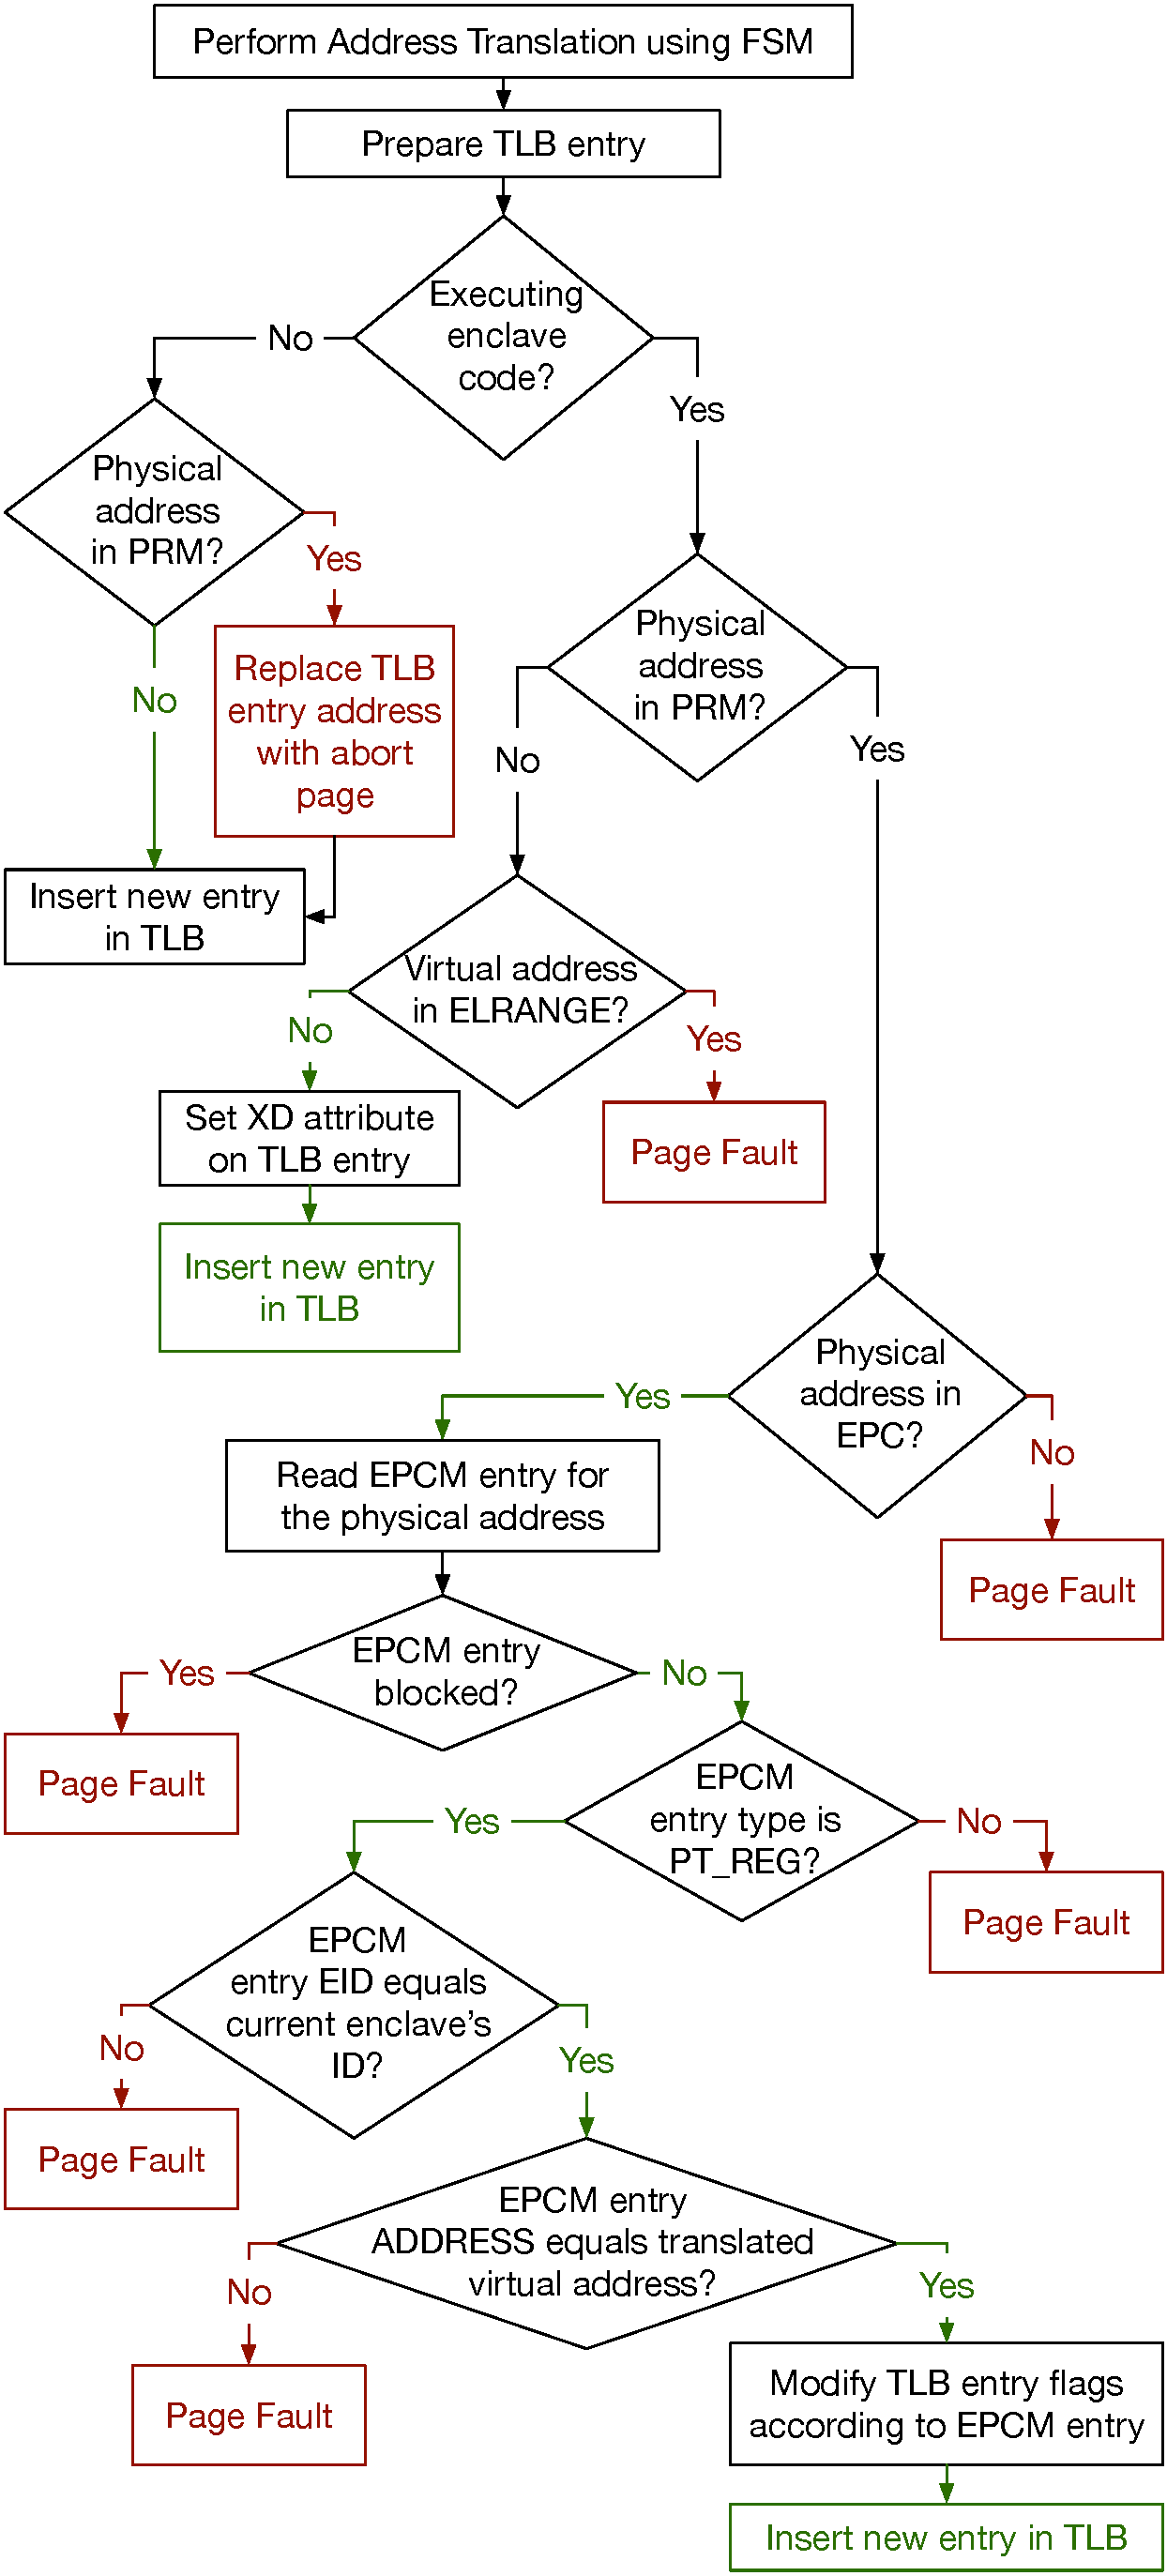
\includegraphics[width=85mm]{figures/sgx_tlb_miss_checks.pdf}
  \caption{
    An enclave's EPC pages are accessed using a dedicated region in the
    enclave's virtual address space, called ELRANGE. The rest of the virtual
    address space maps the host application's memory.
  }
  \label{fig:sgx_tlb_miss_checks}
\end{figure}

% Security Information (SECINFO): SDM S 38.11, S 38.11.{1,2}

The EPCM entry for a page has three access protection bits that must be set to
1 to allow a page to be read (R), written to (W) and executed (X) by enclave
code. When an address translation result points to an EPC page, the access
protection bits in the page's EPCM entry influence the related bits in the
page's TLB entry. For example, if X is 0, the XD bit (\S~\ref{sec:paging}) is
set in the page's TLB entry.

Table~\ref{fig:sgx_pt_values} shows currently defined types. The EPC pages that
store an enclave's code or data have their type set to \textit{regular}
(PT\_REG in the Intel documentation). Each page that is dedicated to an SGX key
data structure has its EPCM entry's type set to the kind of data structure
stored in the page. An EPC page's type is set when the page is allocated, and
is immutable throughout the page's lifetime.

\begin{table}[hbt]
  \centering
  \begin{tabularx}{\columnwidth}{| l | l | X |}
  \hline
  \textbf{Type} & \textbf{Created by} & \textbf{Description}\\
  \hline
  PT\_REG & \texttt{EADD} & enclave code / data \\
  \hline
  PT\_SECS & \texttt{ECREATE} & SECS (\S~\ref{sec:sgx_secs}) \\
  \hline
  PT\_TCS & \texttt{EADD} & TCS (\S~\ref{sec:sgx_tcs}) \\
  \hline
  PT\_VA & \texttt{EPA} & VA (\S~\ref{sec:sgx_va}) \\
  \hline
  \end{tabularx}
  \caption{Values of the PT (page type) field in an EPCM entry.}
  \label{fig:sgx_pt_values}
\end{table}





\subsection {The Implementation of EPC Protection}

The memory controller is
integrated on the CPU die (see Figure~\ref{fig:cpu_die}), so it can be trusted
to prevent devices attached to the system bus from performing DMA transfers
to/from the PRM.

System software manages physical memory by directly modifying the contents of
page tables and EPTs (\S~\ref{sec:paging}), and is responsible for performing
TLB shootdowns (\S~\ref{sec:tlbs}) to ensure that the state not covered by
cache coherence \S~\ref{sec:cache_coherence} is synchronized across logical
processors. If the system software does not perform TLB shootdowns correctly,
application software can experience inconsistent views of memory.

In the context of SGX, an incorrect TLB shootdown can can result in having an
EPC page simultaneously accessible by two different enclaves, which would
compromise the SGX security guarantees. Therefore, the SGX instructions used
for EPC management ensure that the system software performs TLB shootdowns for
the entries that represent EPC pages.


% PRMRR documented in HASP papers and both SGX manuals, completely removed from
% SDM. It still exists in Coreboot. Couldn't find other Skywell code.
The SGX manual states that the EPC (the memory used to store enclave data) can
only be set up as UC or WB. While no further explanation is provided, we assume
that the UC option was provided in order to attempt to mitigate against some
cache-timing attacks.



SECS

% Internal CREGs: SDM S 41.1.4
% ECREATE: SDM S 39.1.1, S 41.3
% EWB: SDM S 41.3

The most important field in the SECS is the 64-bit \textit{enclave ID} (EID),
which is assigned by \texttt{ECREATE}. The EID identifies an enclave's pages in
the EPCM, so it must be unique across all the computer's active enclaves.
According to the ECREATE pseudo-code in the SDM, enclave IDs are allocated
using an atomic counter. An enclave's EID is generally hidden, as most SGX
instructions use the address of the enclave's SECS page as the enclave's
handler. However, the system software can learn an enclave's EID by evicting
one of its EPC pages (\S~\ref{sec:sgx_ewb}).



Currently, the main implication of ELRANGE is that all the SGX data structures
are initialized with enclave virtual addresses specified relatively to
BASEADDR. Furthermore, BASEADDR is not a part of the enclave's measurement
hash (details in \S~\ref{sec:measurement}). It follows that system software can
relocate an enclave in its host application's virtual address space, without
impacting the enclave's measurement hash.

Having ELRANGE follow the memory type range constraints provides a cheap way to
verify if a virtual address belongs to the address, in hardware. This comes in
handy when EENTER has to disable all the hardware breakpoints inside ELRANGE.

An SSA essentially consists of the values of the general-purpose registers
(GPRs), and the result of running XSAVE (\S~\ref{sec:registers}) using the
feature mask specified in the ATTRIBUTES.XFRM field in the enclave's SECS.

Last, the CSSA field in each TCS indicates the next available SSA. When a
logical processor needs to preempt enclave code, it uses the SSA indicated by
the CSSA field, and increments it. The CPU refuses to execute enclave code
using a TCS where no SSA is available (CSSA $\ge$ NSSA).


% Access Control Requirements: SDM S 38.3

Pages that store key SGX structures cannot be accessed directly, even by the
code executing inside their enclaves. Furthermore, the SGX instructions that
operate on SGX data structures check the EPCM type fields of their inputs
against the expected types. This type system prevents software from
intentionally or accidentally corrupting the key SGX data structures.

The type-based access restrictions have the desirable side-effect of hiding the
contents of the EPC pages holding key SGX structures from software, so the
internal layout of any key data structure can change across new CPU revisions.
Software cannot access the key structures in EPC, so it cannot become dependent
on a specific processor's implementation details.

The SGX documentation does specify a software-visible layout for each key data
structure. This layout is used by the non-EPC page used to initialize the key
data structure when it is created. Therefore, new CPU revisions must preserve
the ability to initialize the key data structures from the less flexible
software-visible layout.

